\documentclass[11pt]{article}

%%%% for pictures %%%%
\usepackage{graphicx}
\usepackage{float}

%%% for the degree sign%%%
\usepackage{siunitx}

%%%% for matrices and vectors%%%%

\usepackage{amsmath}

%%%% for citations %%%%%%
\usepackage[backend=biber,
style=apa,
sorting=none,
isbn=true,
doi=true,
url=true,
]{biblatex}\addbibresource{bibliography.bib}

\begin{document}

\title{Fluid Mechanics YouTube}
\author{Theodore Ong}
\date{\today}
\maketitle


\part{Navier Stokes Equations}

Compressible N-S equations
$$\frac{\partial}{\partial t}(\rho \vec{u}) + \nabla \bullet (\rho \vec{u} \otimes \vec{u})  = - \nabla p + \mu \nabla^2 \vec{u} + \frac{1}{3} \mu \nabla (\nabla \bullet \vec{u}) + \rho \vec{g}$$


tensor or outer product:
$$\vec{u} \otimes \vec{v} = \vec{u}\vec{v}^T$$

$$\vec{u}=\begin{pmatrix}
u_1 \\
u_2 \\
u_3 
\end{pmatrix} \ and\ 
\vec{v} = \begin{pmatrix}
v_1 \\
v_2 \\
v_3
\end{pmatrix}
$$


$$ \begin{pmatrix}
u_1 \\
u_2 \\
u_3 
\end{pmatrix} \otimes \begin{pmatrix}
v_1 \\
v_2 \\
v_3 
\end{pmatrix} = \begin{pmatrix}
u_1 \\
u_2 \\
u_3 
\end{pmatrix} \begin{pmatrix}
v_1 && v_2 && v_3
\end{pmatrix}
$$

$$= \begin{pmatrix}
u_1 v_1  && u_1 v_2 && u_1 v_3 \\
u_2  v_1 && u_2 v_2 && u_2 v_3 \\
u_3 v_1 && u_3 v_2 && u_3 v_3
\end{pmatrix}
$$

Inner product

$$\vec{u} \bullet \vec{v} = (\vec{u}^T \vec{v})^T$$


$$ \begin{pmatrix}
u_1 \\
u_2 \\
u_3 
\end{pmatrix} \bullet \begin{pmatrix}
v_1 \\
v_2 \\
v_3 
\end{pmatrix}
=
\begin{pmatrix}
u_1 && u_2 && u_3
\end{pmatrix} \begin{pmatrix}
v_1 \\
v_2 \\
v_3 
\end{pmatrix} $$

$$= u_1 v_1 + u_2 v_2 + u_3 v_3 $$

Assume incompressible flow:

$$\rho=constant$$

continuity equation
$$\nabla \bullet \vec{u}=0$$


Incompressible N-S equations

$$\frac{\partial }{\partial t}\vec{u} +(\vec{u}\bullet \nabla) \vec{u} - \nu \nabla^2 \vec{u} = - \nabla \frac{P}{\rho_0} +\vec{g}$$

\begin{verbatim}
https://en.wikipedia.org/wiki/Navier%E2%80%93Stokes_equations

Matrices in LaTeX
https://www.overleaf.com/learn/latex/Matrices

Tensors in LaTeX

Navier Stokes Equations
https://www.comsol.com/multiphysics/navier-stokes-equations
https://en.wikipedia.org/wiki/Navier%E2%80%93Stokes_equations

Github
https://github.com/theodoreOnzGit/heatTransferTheory_YouTube
\end{verbatim}

First let's deal with:

$$(\vec{u}\bullet \nabla) \vec{u}$$

\begin{equation}
\begin{pmatrix}
\frac{\partial}{\partial x} \\ 
\frac{\partial}{\partial y} \\
\frac{\partial}{\partial z} 
\end{pmatrix} \otimes  \begin{pmatrix}
u_1 \\
u_2 \\
u_3
\end{pmatrix} 
= 
\begin{pmatrix}
\frac{\partial}{\partial x} \\ 
\frac{\partial}{\partial y} \\
\frac{\partial}{\partial z} 
\end{pmatrix}  \begin{pmatrix}
u_1 && u_2 && u_3
\end{pmatrix} 
\end{equation}

$$
= \begin{pmatrix}
\frac{\partial}{\partial x} u_1 && \frac{\partial}{\partial x} u_2 && \frac{\partial}{\partial x} u_3 \\
\frac{\partial}{\partial y} u_1 && \frac{\partial}{\partial y} u_2 && \frac{\partial}{\partial y} u_3 \\
\frac{\partial}{\partial z} u_1 && \frac{\partial}{\partial z} u_2 && \frac{\partial}{\partial z} u_3 
\end{pmatrix}
$$

Then we do inner product

$$
\begin{pmatrix}
u_1 \\
u_2 \\
u_3
\end{pmatrix} \bullet \begin{pmatrix}
\frac{\partial}{\partial x} u_1 && \frac{\partial}{\partial x} u_2 && \frac{\partial}{\partial x} u_3 \\
\frac{\partial}{\partial y} u_1 && \frac{\partial}{\partial y} u_2 && \frac{\partial}{\partial y} u_3 \\
\frac{\partial}{\partial z} u_1 && \frac{\partial}{\partial z} u_2 && \frac{\partial}{\partial z} u_3 
\end{pmatrix} 
$$

$$\begin{pmatrix}
u_1 &&
u_2 &&
u_3
\end{pmatrix} \begin{pmatrix}
\frac{\partial}{\partial x} u_1 && \frac{\partial}{\partial x} u_2 && \frac{\partial}{\partial x} u_3 \\
\frac{\partial}{\partial y} u_1 && \frac{\partial}{\partial y} u_2 && \frac{\partial}{\partial y} u_3 \\
\frac{\partial}{\partial z} u_1 && \frac{\partial}{\partial z} u_2 && \frac{\partial}{\partial z} u_3 
\end{pmatrix}  $$

$$=\begin{pmatrix}
u_1 \frac{\partial}{\partial x} u_1 + u_2 \frac{\partial}{\partial y} u_1 + u_3 \frac{\partial}{\partial z} u_1 \\
u_1 \frac{\partial}{\partial x} u_2 + u_2 \frac{\partial}{\partial y} u_2 + u_3 \frac{\partial}{\partial z} u_2 \\
u_1 \frac{\partial}{\partial x} u_3 + u_2 \frac{\partial}{\partial y} u_3 + u_3 \frac{\partial}{\partial z} u_3
\end{pmatrix}
$$


Let's deal with the momentum diffusivity (kinematic viscosity) term:

$$\nabla^2 = (\nabla \bullet \nabla)$$

$$
\begin{pmatrix}
\frac{\partial}{\partial x} \\ 
\frac{\partial}{\partial y} \\
\frac{\partial}{\partial z} 
\end{pmatrix} \bullet \begin{pmatrix}
\frac{\partial}{\partial x} u_1 && \frac{\partial}{\partial x} u_2 && \frac{\partial}{\partial x} u_3 \\
\frac{\partial}{\partial y} u_1 && \frac{\partial}{\partial y} u_2 && \frac{\partial}{\partial y} u_3 \\
\frac{\partial}{\partial z} u_1 && \frac{\partial}{\partial z} u_2 && \frac{\partial}{\partial z} u_3 
\end{pmatrix} 
$$

$$\begin{pmatrix}
\frac{\partial}{\partial x} &&
\frac{\partial}{\partial y} &&
\frac{\partial}{\partial z} 
\end{pmatrix} \begin{pmatrix}
\frac{\partial}{\partial x} u_1 && \frac{\partial}{\partial x} u_2 && \frac{\partial}{\partial x} u_3 \\
\frac{\partial}{\partial y} u_1 && \frac{\partial}{\partial y} u_2 && \frac{\partial}{\partial y} u_3 \\
\frac{\partial}{\partial z} u_1 && \frac{\partial}{\partial z} u_2 && \frac{\partial}{\partial z} u_3 
\end{pmatrix}  $$

$$=\begin{pmatrix}
\frac{\partial}{\partial x} \frac{\partial}{\partial x} u_1 + \frac{\partial}{\partial y} \frac{\partial}{\partial y} u_1 + \frac{\partial}{\partial z} \frac{\partial}{\partial z} u_1 \\
\frac{\partial}{\partial x} \frac{\partial}{\partial x} u_2 + \frac{\partial}{\partial y} \frac{\partial}{\partial y} u_2 + \frac{\partial}{\partial z} \frac{\partial}{\partial z} u_2 \\
\frac{\partial}{\partial x} \frac{\partial}{\partial x} u_3 + \frac{\partial}{\partial y} \frac{\partial}{\partial y} u_3 + \frac{\partial}{\partial z} \frac{\partial}{\partial z} u_3
\end{pmatrix}
$$


\part{Boundary Layer Equations}

$$\frac{\partial }{\partial t} u + u \frac{\partial}{\partial x} u + v \frac{\partial}{\partial y} u + w \frac{\partial}{\partial z} u - \nu ( \frac{\partial^2}{\partial x^2} u + \frac{\partial^2}{\partial y^2} \ u + \frac{\partial^2}{\partial z^2} u) = - \frac{1}{\rho_0} \frac{\partial P}{\partial x} +g_x$$

$$\frac{\partial }{\partial t} v + u \frac{\partial}{\partial x} v + v \frac{\partial}{\partial y} v + w \frac{\partial}{\partial z} v - \nu ( \frac{\partial^2}{\partial x^2} v + \frac{\partial^2}{\partial y^2} \ v + \frac{\partial^2}{\partial z^2} v) = - \frac{1}{\rho_0} \frac{\partial P}{\partial y} +g_y$$

$$\frac{\partial }{\partial t} w + u \frac{\partial}{\partial x} w + v \frac{\partial}{\partial y} w + w \frac{\partial}{\partial z} w - \nu ( \frac{\partial^2}{\partial x^2} w + \frac{\partial^2}{\partial y^2} \ w + \frac{\partial^2}{\partial z^2} w) = - \frac{1}{\rho_0} \frac{\partial P}{\partial z} +g_z$$

Now for 2D what do we do?
w=0 everywhere and at all times, $g_z=0$

We eliminate z terms from the x and y momentum balance

$$\frac{\partial }{\partial t} u + u \frac{\partial}{\partial x} u + v \frac{\partial}{\partial y} u - \nu ( \frac{\partial^2}{\partial x^2} u + \frac{\partial^2}{\partial y^2} \ u + \frac{\partial^2}{\partial z^2} u) = - \frac{1}{\rho_0} \frac{\partial P}{\partial x} +g_x$$

$$\frac{\partial }{\partial t} v + u \frac{\partial}{\partial x} v + v \frac{\partial}{\partial y} v - \nu ( \frac{\partial^2}{\partial x^2} v + \frac{\partial^2}{\partial y^2} \ v + \frac{\partial^2}{\partial z^2} v) = - \frac{1}{\rho_0} \frac{\partial P}{\partial y} +g_y$$

There is no spatial variation in u and v w.r.t z
We have 2D Navier stokes:

$$\frac{\partial }{\partial t} u + u \frac{\partial}{\partial x} u + v \frac{\partial}{\partial y} u - \nu ( \frac{\partial^2}{\partial x^2} u + \frac{\partial^2}{\partial y^2} \ u ) = - \frac{1}{\rho_0} \frac{\partial P}{\partial x} +g_x$$

$$\frac{\partial }{\partial t} v + u \frac{\partial}{\partial x} v + v \frac{\partial}{\partial y} v - \nu ( \frac{\partial^2}{\partial x^2} v + \frac{\partial^2}{\partial y^2} \ v ) = - \frac{1}{\rho_0} \frac{\partial P}{\partial y} +g_y$$

continuity equation

$$\frac{\partial }{\partial x} u + \frac{\partial}{\partial y} v + \frac{\partial}{\partial z} w=0$$

$$\frac{\partial }{\partial x} u + \frac{\partial}{\partial y} v =0 $$

\section{nondimensionalisation}
Order of magnitude
$$\mathcal{O}$$

Scaling for order magnitude comparison 

$$u^* , y^* =\mathcal{O}(1)$$


we define:
$$u^* = \frac{u}{u_\infty}$$
$$u = u_\infty u^*$$

$$x^* = \frac{x}{L}$$

$$y^* = \frac{y}{\delta_p}$$

We scale our continutity equation:

$$\frac{\partial }{\partial x^* L} u^* u_\infty + \frac{\partial}{\partial y^* \delta_p} v =0 $$

$$\frac{\partial }{\partial x^* L} u^* u_\infty + \frac{\partial}{\partial y^* \delta_p} v =0 $$

$$ \frac{u_\infty}{L} \frac{\partial }{\partial x^* } u^* + \frac{1}{\delta_p}\frac{\partial}{\partial y^*} v =0 $$


$$\frac{\partial }{\partial x^* } u^* + \frac{L}{\delta_p u_\infty}\frac{\partial}{\partial y^*} v =0 $$

$$v^*=\frac{vL}{\delta_p u_\infty}=  \mathcal{O}(1)$$

$$v^* = \frac{v}{\frac{u_\infty \delta_p}{L}}$$

$$\frac{\partial }{\partial x^* } u^* + \frac{\partial}{\partial y^*} v^* =0 $$

Now we move on to the NS equations

so we need to scale time:

x lengthscale = L

x velocityscale = $u_\infty$

timescale = $\frac{L}{u_\infty}$

$$t^* = \frac{t}{\frac{L}{u_\infty}}$$

Let's scale the momentum NS equations 

$$\frac{\partial }{\partial t} u + u \frac{\partial}{\partial x} u + v \frac{\partial}{\partial y} u - \nu ( \frac{\partial^2}{\partial x^2} u + \frac{\partial^2}{\partial y^2} \ u ) = - \frac{1}{\rho_0} \frac{\partial P}{\partial x} +g_x$$

$$\frac{\partial }{\partial t} v + u \frac{\partial}{\partial x} v + v \frac{\partial}{\partial y} v - \nu ( \frac{\partial^2}{\partial x^2} v + \frac{\partial^2}{\partial y^2} \ v ) = - \frac{1}{\rho_0} \frac{\partial P}{\partial y} +g_y$$

Let's do x momentum equations

$$\frac{\partial }{\partial t} u^* u_\infty + u^* u_\infty \frac{\partial}{\partial x^* L} u^* u_\infty + v \frac{\partial}{\partial y} u^* u_\infty - \nu ( \frac{\partial^2}{\partial x^2} u^* u_\infty + \frac{\partial^2}{\partial y^2} \ u^* u_\infty ) = - \frac{1}{\rho_0} \frac{\partial P}{\partial x} +g_x$$


$$\frac{\partial }{\partial t} u^* + u^* \frac{u_\infty}{L} \frac{\partial}{\partial x^* } u^* + v \frac{1}{\delta_p} \frac{\partial}{\partial y^*} u^* - \nu (\frac{1}{L^2} \frac{\partial^2}{\partial (x^*)^2} u^* + \frac{1}{\delta_p^2} \frac{\partial^2}{\partial (y^*)^2} \ u^* ) = \frac{1}{u_\infty} ( - \frac{1}{L \rho_0} \frac{\partial P}{\partial x^*} +g_x)$$

$$\frac{u_\infty}{L}\frac{\partial }{\partial t^*} u^* + u^* \frac{u_\infty}{L} \frac{\partial}{\partial x^* } u^* + v \frac{1}{\delta_p} \frac{\partial}{\partial y^*} u^* - \nu (\frac{1}{L^2} \frac{\partial^2}{\partial (x^*)^2} u^* + \frac{1}{\delta_p^2} \frac{\partial^2}{\partial (y^*)^2} \ u^* ) = \frac{1}{u_\infty} ( - \frac{1}{L \rho_0} \frac{\partial P}{\partial x^*} +g_x)$$


$$\frac{\partial }{\partial t^*} u^* + u^*  \frac{\partial}{\partial x^* } u^* + v^*  \frac{\partial}{\partial y^*} u^* - \frac{\nu}{u_\infty L}  ( \frac{\partial^2}{\partial (x^*)^2} u^* + \frac{L^2}{\delta_p^2} \frac{\partial^2}{\partial (y^*)^2} \ u^* ) = \frac{L}{u_\infty^2} ( - \frac{1}{L \rho_0} \frac{\partial P}{\partial x^*} +g_x)$$

Reynold's number
$$Re_L  = \frac{u_\infty L}{\nu}$$

$$\frac{\partial }{\partial t^*} u^* + u^*  \frac{\partial}{\partial x^* } u^* + v^*  \frac{\partial}{\partial y^*} u^* - \frac{1}{Re_L}  ( \frac{\partial^2}{\partial (x^*)^2} u^* + \frac{L^2}{\delta_p^2} \frac{\partial^2}{\partial (y^*)^2} \ u^* ) = \frac{L}{u_\infty^2} ( - \frac{1}{L \rho_0} \frac{\partial P}{\partial x^*} +g_x)$$

$$\frac{\partial }{\partial t^*} u^* + u^*  \frac{\partial}{\partial x^* } u^* + v^*  \frac{\partial}{\partial y^*} u^* - \frac{1}{Re_L}  ( \frac{\partial^2}{\partial (x^*)^2} u^* + \frac{L^2}{\delta_p^2} \frac{\partial^2}{\partial (y^*)^2} \ u^* ) =  ( - \frac{1}{L \rho_0}  \frac{L}{u_\infty^2} \frac{\partial P}{\partial x^*} + \frac{L}{u_\infty^2}g_x)$$

Let's scale gravity

$$g_x^* = \frac{g_x}{|g|} = \cos \theta_x = \mathcal{O}(1)$$


$$\frac{\partial }{\partial t^*} u^* + u^*  \frac{\partial}{\partial x^* } u^* + v^*  \frac{\partial}{\partial y^*} u^* - \frac{1}{Re_L}  ( \frac{\partial^2}{\partial (x^*)^2} u^* + \frac{L^2}{\delta_p^2} \frac{\partial^2}{\partial (y^*)^2} \ u^* ) =  ( -  \frac{1}{ \rho_0 u_\infty^2} \frac{\partial P}{\partial x^*} + \frac{L |g|}{u_\infty^2}g_x^* )$$


$$\frac{\partial }{\partial t^*} u^* + u^*  \frac{\partial}{\partial x^* } u^* + v^*  \frac{\partial}{\partial y^*} u^* - \frac{1}{Re_L}  ( \frac{\partial^2}{\partial (x^*)^2} u^* + \frac{L^2}{\delta_p^2} \frac{\partial^2}{\partial (y^*)^2} \ u^* ) =  ( -  \frac{1}{ \rho_0 u_\infty^2} \frac{\partial P}{\partial x^*} + \frac{1}{Fr^2}g_x^* )$$


$$P^* = \frac{P}{\rho_0 u_\infty^2}$$

After nondimensionalisation, our x momentum equation becomes:

$$\frac{\partial }{\partial t^*} u^* + u^*  \frac{\partial}{\partial x^* } u^* + v^*  \frac{\partial}{\partial y^*} u^* - \frac{1}{Re_L}  ( \frac{\partial^2}{\partial (x^*)^2} u^* + \frac{L^2}{\delta_p^2} \frac{\partial^2}{\partial (y^*)^2} \ u^* ) =  ( -  \frac{\partial P^*}{\partial x^*} + \frac{1}{Fr^2}g_x^* )$$

we dimensionalise y momentum eqns

$$\frac{\partial }{\partial t} v + u \frac{\partial}{\partial x} v + v \frac{\partial}{\partial y} v - \nu ( \frac{\partial^2}{\partial x^2} v + \frac{\partial^2}{\partial y^2} \ v ) = - \frac{1}{\rho_0} \frac{\partial P}{\partial y} +g_y$$

First the x and time terms:
$$ \frac{u_\infty}{L} \frac{\partial }{\partial t^*} v + u^* \frac{u_\infty}{L} \frac{\partial}{\partial x^*} v + v \frac{\partial}{\partial y} v - \nu (\frac{1}{L^2} \frac{\partial^2}{\partial (x^*)^2} v + \frac{\partial^2}{\partial y^2} \ v ) = - \frac{1}{\rho_0} \frac{\partial P}{\partial y} +g_y$$

Second y coordinate terms:
$$ \frac{u_\infty}{L} \frac{\partial }{\partial t^*} v + u^* \frac{u_\infty}{L} \frac{\partial}{\partial x^*} v + v \frac{1}{\delta_p} \frac{\partial}{\partial y^*} v - \nu (\frac{1}{L^2} \frac{\partial^2}{\partial (x^*)^2} v + \frac{1}{\delta_p^2} \frac{\partial^2}{\partial (y^*)^2} \ v ) = - \frac{1}{\rho_0} \frac{1}{\delta_p} \frac{\partial P}{\partial y^*} +g_y^*|g|$$

divide by $\frac{u_\infty^2}{L^2}$

$$ \frac{L}{u_\infty} \frac{\partial }{\partial t^*} v + u^* \frac{L}{u_\infty} \frac{\partial}{\partial x^*} v + v \frac{L^2}{ u_\infty^2 \delta_p} \frac{\partial}{\partial y^*} v - \nu \frac{L^2}{u_\infty^2} (\frac{1}{L^2} \frac{\partial^2}{\partial (x^*)^2} v + \frac{1}{\delta_p^2} \frac{\partial^2}{\partial (y^*)^2} \ v ) =  \frac{L^2}{u_\infty^2}(- \frac{1}{\rho_0} \frac{1}{\delta_p} \frac{\partial P}{\partial y^*} +g_y^* |g|)$$

divide by $\delta_p$

$$ \frac{L }{u_\infty \delta_p} \frac{\partial }{\partial t^*} v + u^* \frac{L }{u_\infty \delta_p} \frac{\partial}{\partial x^*} v + v \frac{L^2}{ u_\infty^2 \delta_p^2} \frac{\partial}{\partial y^*} v - \nu \frac{L^2}{u_\infty^2 \delta_p } (\frac{1}{L^2} \frac{\partial^2}{\partial (x^*)^2} v + \frac{1}{\delta_p^2} \frac{\partial^2}{\partial (y^*)^2} \ v ) =  \frac{L^2 }{u_\infty^2 \delta_p}(- \frac{1}{\rho_0} \frac{1}{\delta_p} \frac{\partial P}{\partial y^*} +g_y^* |g|)$$


Combining some terms
$$  \frac{\partial }{\partial t^*} v^* + u^*  \frac{\partial}{\partial x^*} v^* + v^* \frac{\partial}{\partial y^*} v^* - \nu \frac{L}{u_\infty  } (\frac{1}{L^2} \frac{\partial^2}{\partial (x^*)^2} v^* + \frac{1}{\delta_p^2} \frac{\partial^2}{\partial (y^*)^2} \ v^* ) =  \frac{L^2 }{u_\infty^2 \delta_p}(- \frac{1}{\rho_0} \frac{1}{\delta_p} \frac{\partial P}{\partial y^*} +g_y^* |g|)$$

Rearranging

$$  \frac{\partial }{\partial t^*} v^* + u^*  \frac{\partial}{\partial x^*} v^* + v^* \frac{\partial}{\partial y^*} v^* -  \frac{\nu}{u_\infty L } ( \frac{\partial^2}{\partial (x^*)^2} v^* + \frac{L^2}{\delta_p^2} \frac{\partial^2}{\partial (y^*)^2} \ v^* ) =  (- \frac{1}{\rho_0}\frac{L^2 }{u_\infty^2 \delta_p} \frac{1}{\delta_p} \frac{\partial P}{\partial y^*} +g_y^* |g|\frac{L^2 }{u_\infty^2 \delta_p})$$

nondimensionalisng pressure and including the Fr

$$  \frac{\partial }{\partial t^*} v^* + u^*  \frac{\partial}{\partial x^*} v^* + v^* \frac{\partial}{\partial y^*} v^* -  \frac{\nu}{u_\infty L } ( \frac{\partial^2}{\partial (x^*)^2} v^* + \frac{L^2}{\delta_p^2} \frac{\partial^2}{\partial (y^*)^2} \ v^* ) =  (- \frac{L^2 }{\delta_p^2} \frac{\partial P^*}{\partial y^*} +g_y^*\frac{1}{Fr^2}\frac{L }{ \delta_p})$$

Include Re

$$  \frac{\partial }{\partial t^*} v^* + u^*  \frac{\partial}{\partial x^*} v^* + v^* \frac{\partial}{\partial y^*} v^* -  \frac{1}{Re_L } ( \frac{\partial^2}{\partial (x^*)^2} v^* + \frac{L^2}{\delta_p^2} \frac{\partial^2}{\partial (y^*)^2} \ v^* ) =  (- \frac{L^2 }{\delta_p^2} \frac{\partial P^*}{\partial y^*} +g_y^*\frac{1}{Fr^2}\frac{L }{ \delta_p})$$


Review: NS nondimensionalised

$$\frac{\partial }{\partial t^*} u^* + u^*  \frac{\partial}{\partial x^* } u^* + v^*  \frac{\partial}{\partial y^*} u^* - \frac{1}{Re_L}  ( \frac{\partial^2}{\partial (x^*)^2} u^* + \frac{L^2}{\delta_p^2} \frac{\partial^2}{\partial (y^*)^2} \ u^* ) =  ( -  \frac{\partial P^*}{\partial x^*} + \frac{1}{Fr^2}g_x^* )$$


$$  \frac{\partial }{\partial t^*} v^* + u^*  \frac{\partial}{\partial x^*} v^* + v^* \frac{\partial}{\partial y^*} v^* -  \frac{1}{Re_L } ( \frac{\partial^2}{\partial (x^*)^2} v^* + \frac{L^2}{\delta_p^2} \frac{\partial^2}{\partial (y^*)^2} \ v^* ) =  (- \frac{L^2 }{\delta_p^2} \frac{\partial P^*}{\partial y^*} +g_y^*\frac{1}{Fr^2}\frac{L }{ \delta_p})$$

$$\frac{\partial }{\partial x^* } u^* + \frac{\partial}{\partial y^*} v^* =0 $$

\section{How to drop terms?}

$$\frac{\partial }{\partial t^*} u^* + u^*  \frac{\partial}{\partial x^* } u^* + v^*  \frac{\partial}{\partial y^*} u^* - \frac{1}{Re_L}  ( \frac{\partial^2}{\partial (x^*)^2} u^* + \frac{L^2}{\delta_p^2} \frac{\partial^2}{\partial (y^*)^2} \ u^* ) =  ( -  \frac{\partial P^*}{\partial x^*} + \frac{1}{Fr^2}g_x^* )$$


$$  \frac{\partial }{\partial t^*} v^* + u^*  \frac{\partial}{\partial x^*} v^* + v^* \frac{\partial}{\partial y^*} v^* -  \frac{1}{Re_L } ( \frac{\partial^2}{\partial (x^*)^2} v^* + \frac{L^2}{\delta_p^2} \frac{\partial^2}{\partial (y^*)^2} \ v^* ) =  (- \frac{L^2 }{\delta_p^2} \frac{\partial P^*}{\partial y^*} +g_y^*\frac{1}{Fr^2}\frac{L }{ \delta_p})$$

$$\frac{\partial }{\partial x^* } u^* + \frac{\partial}{\partial y^*} v^* =0 $$

When we want to determine which terms to cancel, we need to know how $Re_L$ compares with $\frac{L^2}{\delta_p^2}$

Assumption:

Creeping flow in y direction

$$Re_\delta = \frac{v_c \delta_p}{\nu} = \mathcal{O}(1)$$

How does $Re_\delta$ compare to $Re_L$

$$v_c = u_\infty \frac{\delta_p}{L}$$

$$Re_\delta = \frac{u_\infty \frac{\delta_p}{L} \delta_p}{\nu} = \mathcal{O}(1)$$

$$Re_\delta = \frac{u_\infty  L}{\nu} \frac{\delta_p^2}{L^2} = \mathcal{O}(1)$$

$$Re_\delta = Re_L \frac{\delta_p^2}{L^2} = \mathcal{O}(1)$$

\subsubsection{x direction momentum eqn}

$$\frac{\partial }{\partial t^*} u^* + u^*  \frac{\partial}{\partial x^* } u^* + v^*  \frac{\partial}{\partial y^*} u^* - \frac{1}{Re_L}  ( \frac{\partial^2}{\partial (x^*)^2} u^* + \frac{L^2}{\delta_p^2} \frac{\partial^2}{\partial (y^*)^2} \ u^* ) =  ( -  \frac{\partial P^*}{\partial x^*} + \frac{1}{Fr^2}g_x^* )$$

$$\frac{\partial }{\partial t^*} u^* + u^*  \frac{\partial}{\partial x^* } u^* + v^*  \frac{\partial}{\partial y^*} u^* -   \frac{1}{Re_L} \frac{\partial^2}{\partial (x^*)^2} u^* + \frac{1}{Re_L} \frac{L^2}{\delta_p^2} \frac{\partial^2}{\partial (y^*)^2} \ u^*  =  ( -  \frac{\partial P^*}{\partial x^*} + \frac{1}{Fr^2}g_x^* )$$

$$\frac{\partial }{\partial t^*} u^* + u^*  \frac{\partial}{\partial x^* } u^* + v^*  \frac{\partial}{\partial y^*} u^* -   \frac{1}{Re_L} \frac{\partial^2}{\partial (x^*)^2} u^* + \frac{1}{\mathcal{O}(1)} \frac{\partial^2}{\partial (y^*)^2} \ u^*  =  ( -  \frac{\partial P^*}{\partial x^*} + \frac{1}{Fr^2}g_x^* )$$

How big is $Re_L$?

$$Re_L = \mathcal{O} (\frac{L^2}{\delta_p^2})$$

We assume Fr is big 

$$\frac{\partial }{\partial t^*} u^* + u^*  \frac{\partial}{\partial x^* } u^* + v^*  \frac{\partial}{\partial y^*} u^* -  + \frac{1}{\mathcal{O}(1)} \frac{\partial^2}{\partial (y^*)^2} \ u^*  =  ( -  \frac{\partial P^*}{\partial x^*} )$$

\subsubsection{y direction momentum equation}

$$  \frac{\partial }{\partial t^*} v^* + u^*  \frac{\partial}{\partial x^*} v^* + v^* \frac{\partial}{\partial y^*} v^* -  \frac{1}{Re_L } ( \frac{\partial^2}{\partial (x^*)^2} v^* + \frac{L^2}{\delta_p^2} \frac{\partial^2}{\partial (y^*)^2} \ v^* ) =  (- \frac{L^2 }{\delta_p^2} \frac{\partial P^*}{\partial y^*} +g_y^*\frac{1}{Fr^2}\frac{L }{ \delta_p})$$


$$  \frac{\partial }{\partial t^*} v^* + u^*  \frac{\partial}{\partial x^*} v^* + v^* \frac{\partial}{\partial y^*} v^* -   ( \frac{1}{Re_L } \frac{\partial^2}{\partial (x^*)^2} v^* +  \frac{1}{\mathcal{O}(1) } \frac{\partial^2}{\partial (y^*)^2} \ v^* ) =  (- \frac{L^2 }{\delta_p^2} \frac{\partial P^*}{\partial y^*} +g_y^*\frac{1}{Fr^2}\frac{L }{ \delta_p})$$

$$  [\frac{\partial }{\partial t^*} v^* + u^*  \frac{\partial}{\partial x^*} v^* + v^* \frac{\partial}{\partial y^*} v^* ] \frac{1}{Re_L}-   ( \frac{1}{Re_L^2 } \frac{\partial^2}{\partial (x^*)^2} v^* +  \frac{1}{\mathcal{O}(1) Re_L} \frac{\partial^2}{\partial (y^*)^2} \ v^* ) =  \frac{1}{Re_L}(- \frac{L^2 }{\delta_p^2} \frac{\partial P^*}{\partial y^*} +g_y^*\frac{1}{Fr^2}\frac{L }{ \delta_p})$$

$$  [\frac{\partial }{\partial t^*} v^* + u^*  \frac{\partial}{\partial x^*} v^* + v^* \frac{\partial}{\partial y^*} v^* ] \frac{1}{Re_L}-   ( \frac{1}{Re_L^2 } \frac{\partial^2}{\partial (x^*)^2} v^* +  \frac{1}{\mathcal{O}(1) Re_L} \frac{\partial^2}{\partial (y^*)^2} \ v^* )$$

$$ =  (- \frac{L^2 }{\delta_p^2} \frac{1}{Re_L}\frac{\partial P^*}{\partial y^*} +g_y^*\frac{1}{Fr^2}\frac{L }{ \delta_p}\frac{1}{Re_L})$$

Cancelling out...

$$  [\frac{\partial }{\partial t^*} v^* + u^*  \frac{\partial}{\partial x^*} v^* + v^* \frac{\partial}{\partial y^*} v^* ] \frac{1}{Re_L}-   ( \frac{1}{Re_L^2 } \frac{\partial^2}{\partial (x^*)^2} v^* +  \frac{1}{\mathcal{O}(1) Re_L} \frac{\partial^2}{\partial (y^*)^2} \ v^* )$$

$$ =  (- \frac{1}{\mathcal{O}(1)}\frac{\partial P^*}{\partial y^*} +g_y^*\frac{1}{Fr^2}\frac{L^2 }{ \delta_p^2}\frac{1}{Re_L} \frac{\delta_p}{L})$$


Simplifying

$$  [\frac{\partial }{\partial t^*} v^* + u^*  \frac{\partial}{\partial x^*} v^* + v^* \frac{\partial}{\partial y^*} v^* ] \frac{1}{Re_L}-   ( \frac{1}{Re_L^2 } \frac{\partial^2}{\partial (x^*)^2} v^* +  \frac{1}{\mathcal{O}(1) Re_L} \frac{\partial^2}{\partial (y^*)^2} \ v^* )$$

$$ =  \frac{1}{\mathcal{O}(1)} (-\frac{\partial P^*}{\partial y^*} +g_y^*\frac{1}{Fr^2}\frac{\delta_p}{L})$$

For large $Re_L$

$$0 =  (-\frac{\partial P^*}{\partial y^*} +g_y^*\frac{1}{Fr^2}\frac{\delta_p}{L})$$

$$g_y^*\frac{1}{Fr^2}\frac{\delta_p}{L} =  \frac{\partial P^*}{\partial y^*} $$

Only if g=0,

$$0 = - \frac{\partial P^*}{\partial y^*} $$

Now we have our BL equations:
$$0 = - \frac{\partial P^*}{\partial y^*} $$


$$\frac{\partial }{\partial t^*} u^* + u^*  \frac{\partial}{\partial x^* } u^* + v^*  \frac{\partial}{\partial y^*} u^* - \frac{1}{\mathcal{O}(1)} \frac{\partial^2}{\partial (y^*)^2} \ u^*  =  ( -  \frac{\partial P^*}{\partial x^*} )$$

redimensionalise to obtain the laminar BL equations:
$$0 = - \frac{\partial P}{\partial y} $$

$$\frac{\partial }{\partial t} u + u  \frac{\partial}{\partial x } u + v  \frac{\partial}{\partial y} u -  \nu  \frac{\partial^2}{\partial (y)^2} \ u  =  ( -  \frac{\partial P}{\partial x} )$$

$$\frac{\partial u}{\partial x} + \frac{\partial v}{\partial y} = 0$$

\section{Solutions to the BL equations laminar}
How to solve?
\begin{itemize}
\item 1st Similarity solution
\item 2nd Von Karman Solution (Integral solution - approximate)
\item 3rd numerical (CFD)
\end{itemize}

\subsection{similarity solution (Blasius solution)}
$$0 = - \frac{\partial P}{\partial y} $$

$$\frac{\partial }{\partial t} u + u  \frac{\partial}{\partial x } u + v  \frac{\partial}{\partial y} u -  \nu  \frac{\partial^2}{\partial (y)^2} \ u  =  ( -  \frac{\partial P}{\partial x} )$$

$$\frac{\partial u}{\partial x} + \frac{\partial v}{\partial y} = 0$$

Similarity solution $\rightarrow$ combine variables to convert PDE to ODE

Making 2 assumptions before we continue:

1) steady state
2) no pressure gradient

$$ u  \frac{\partial}{\partial x } u + v  \frac{\partial}{\partial y} u -  \nu  \frac{\partial^2}{\partial y^2} \ u  =  0$$

$$\frac{\partial u}{\partial x} + \frac{\partial v}{\partial y} = 0$$

How to combine variables to make life easier for us to solve?

introduce the streamfunction ($\psi$):

$$u = \frac{\partial \psi}{\partial y}$$
$$v = -\frac{\partial \psi}{\partial x}$$

Note: streamfunction only works for 2D fluid flow

Substitute into 2D continuity equation,

$$\frac{\partial}{\partial x} \frac{\partial \psi}{\partial y} - \frac{\partial}{\partial y}  \frac{\partial \psi}{\partial x}= 0$$

Substitute into the 2D x momentum equation

$$ (\frac{\partial \psi}{\partial y})  \frac{\partial}{\partial x } (\frac{\partial \psi}{\partial y}) + (-\frac{\partial \psi}{\partial x})  \frac{\partial}{\partial y} (\frac{\partial \psi}{\partial y}) -  \nu  \frac{\partial^2}{\partial y^2} (\frac{\partial \psi}{\partial y})  =  0$$


$$ (\frac{\partial \psi}{\partial y})  \frac{\partial}{\partial x } (\frac{\partial \psi}{\partial y}) - (\frac{\partial \psi}{\partial x})  (\frac{\partial^2 \psi}{\partial y^2}) -  \nu  \frac{\partial^3}{\partial y^3} \psi  =  0$$

We need to compress the number of variables further to 1 indep variable ($\eta$) and 1 dependent variable (f($\eta$))

$$\eta= \eta(x,y)$$

$$f= f(\eta)$$

Before we continue, BCs first!

1 BC in x dir for u

$$x=0 , y\neq 0, u=u_\infty$$

2 BCs in y dir for u 

no slip
$$u=0 \ at \ y=0$$
$$y \rightarrow \infty;\ u \rightarrow u_\infty$$
1 BC in y direction for v

no slip
$$v=0 \ at \ y=0$$

\subsubsection{similarity transform}

How do we start to get these "combo parameters" aka similarity variables?

\begin{verbatim}
https://ntrs.nasa.gov/citations/20050028493
\end{verbatim}

Based on Blasius's paper (translated by NACA) it's good to nondimnesionalise to find these similarity variables

$$\psi^* = \frac{\psi}{\psi_0}$$

Let's nondimensionalise the momentum equations:

$$ (\frac{\partial \psi}{\partial y})  \frac{\partial}{\partial x } (\frac{\partial \psi}{\partial y}) - (\frac{\partial \psi}{\partial x})  (\frac{\partial^2 \psi}{\partial y^2}) -  \nu  \frac{\partial^3}{\partial y^3} \psi  =  0$$

$$ \frac{\psi_0^2}{\delta_p^2 L}  (\frac{\partial \psi^*}{\partial y^*})  \frac{\partial}{\partial x^* } (\frac{\partial \psi^*}{\partial y^*}) - \frac{\psi_0^2}{L \delta_p^2} (\frac{\partial \psi^*}{\partial x^*})  (\frac{\partial^2 \psi^*}{\partial (y^*)^2}) -  \frac{\nu \psi_0}{\delta_p^3} \frac{\partial^3}{\partial (y^*)^3} \psi^*  =  0$$


$$  (\frac{\partial \psi^*}{\partial y^*})  \frac{\partial}{\partial x^* } (\frac{\partial \psi^*}{\partial y^*}) - (\frac{\partial \psi^*}{\partial x^*})  (\frac{\partial^2 \psi^*}{\partial (y^*)^2}) -  \frac{\nu \psi_0}{\delta_p^3} \frac{\delta_p^2 L}{\psi_0^2} \frac{\partial^3}{\partial (y^*)^3} \psi^*  =  0$$

$$  (\frac{\partial \psi^*}{\partial y^*})  \frac{\partial}{\partial x^* } (\frac{\partial \psi^*}{\partial y^*}) - (\frac{\partial \psi^*}{\partial x^*})  (\frac{\partial^2 \psi^*}{\partial (y^*)^2}) -  \frac{\nu }{\delta_p} \frac{ L}{\psi_0} \frac{\partial^3}{\partial (y^*)^3} \psi^*  =  0$$

dimensionless group:

$$\frac{\nu L }{\delta_p \psi_0} = \mathcal{O}(1)$$

We want the equations to be nondimensionalised exactly.

If we want the equations looks like:

$$  (\frac{\partial \psi^*}{\partial y^*})  \frac{\partial}{\partial x^* } (\frac{\partial \psi^*}{\partial y^*}) - (\frac{\partial \psi^*}{\partial x^*})  (\frac{\partial^2 \psi^*}{\partial (y^*)^2}) - \frac{\partial^3}{\partial (y^*)^3} \psi^*  =  0$$

$$\frac{\nu L }{\delta_p \psi_0} = 1$$

$$\psi_0 = \frac{\nu L}{\delta_p}$$

Otherwise:

$$\psi_0 = \mathcal{O}(1) \frac{\nu L}{\delta_p} $$

How do we get rid of dependent variables $\delta_p$?

$$Re_\delta = \frac{v_c \delta_p}{\nu}=\mathcal{O}(1)$$

$$Re_\delta = \frac{u_\infty L}{\nu} \frac{\delta_p^2}{L^2} = \mathcal{O}(1)$$

From continutity equation 

$$v_c = \frac{u_\infty \delta_p}{L}$$

(not too helpful)

What's helpful is to use the physics of the BL ie creeping flow in BL

The other assumption: 

$$Re_\delta = 1$$

$$Re_\delta = \frac{u_\infty }{\nu L}\delta_p^2$$

$$\delta_p  = \sqrt{Re_\delta} \sqrt{\frac{\nu L}{u_\infty}}$$

Substitute back:

$$\psi_0 = \frac{\nu L}{\delta_p}=\frac{\nu L}{\sqrt{Re_\delta} \sqrt{\frac{\nu L}{u_\infty}}} $$

$$\psi_0 =\frac{\nu L}{ \sqrt{\frac{\nu L}{u_\infty}}} \frac{1}{\sqrt{Re_\delta}} $$


$$\psi_0 = \sqrt{u_\infty L \nu} \frac{1}{\sqrt{Re_\delta}} $$

Let's see our nondimensionalised streamfunction:

$$\psi^* = \frac{\psi}{\psi_0} = \sqrt{Re_\delta} \frac{\psi}{\sqrt{u_\infty L \nu }} $$

If $Re_\delta=1$

$$\psi^* = \frac{\psi}{\psi_0} = \frac{\psi}{\sqrt{u_\infty L \nu }} $$

What about our independent variable? We need to combine the x and y coordinate variables

we'll use 


$$Re_\delta = \frac{u_\infty }{\nu L}\delta_p^2$$

$$\delta_p  = \sqrt{Re_\delta} \sqrt{\frac{\nu L}{u_\infty}}$$

If we want x and y explicitly, 

$$x = x^* L$$

$$y=y^* \delta_p$$

$$ \frac{y}{y^*} = \sqrt{Re_\delta} \sqrt{\frac{\nu \frac{x}{x^*}}{u_\infty}}$$

$$ y = \sqrt{Re_\delta} \frac{y^*}{\sqrt{x^*}} \sqrt{\frac{\nu x}{u_\infty}}$$

$$ y = \sqrt{Re_\delta} \frac{y^*}{\sqrt{x^*}} \sqrt{\frac{\nu x}{u_\infty}}$$

$$y \sqrt{\frac{u_\infty}{\nu x}} = \sqrt{Re_\delta} \frac{y^*}{\sqrt{x^*}} = \mathcal{O}(1)$$

And we have dimensionless stream function

$$\psi^* = \frac{\psi}{\psi_0} = \frac{\psi}{\sqrt{u_\infty L \nu }} $$


$$\psi^* = \frac{\psi}{\sqrt{u_\infty \frac{x}{x^*} \nu }} $$
$$\psi^* = \sqrt{x^*}\frac{\psi}{\sqrt{u_\infty x \nu }} $$

If $Re_{\delta} \neq 1$

$$\psi^* = \frac{\psi}{\psi_0} = \sqrt{Re_\delta} \frac{\psi}{\sqrt{u_\infty L \nu }} $$

$$\psi^* = \frac{\psi}{\psi_0} = \sqrt{Re_\delta x^*} \frac{\psi}{\sqrt{u_\infty x \nu }} $$


from Blasius's paper:
$$\eta = \frac{1}{2} \sqrt{Re_\delta} \frac{y^*}{\sqrt{x^*}} = \frac{1}{2}y \sqrt{\frac{u_\infty}{\nu x}} $$

$$f(\eta) = \frac{\psi^*}{\sqrt{x^* Re_\delta}} = \frac{\psi}{\sqrt{u_\infty x \nu}}$$

We start transforming variables

$$  (\frac{\partial \psi^*}{\partial y^*})  \frac{\partial}{\partial x^* } (\frac{\partial \psi^*}{\partial y^*}) - (\frac{\partial \psi^*}{\partial x^*})  (\frac{\partial^2 \psi^*}{\partial (y^*)^2}) - \frac{\partial^3}{\partial (y^*)^3} \psi^*  =  0$$


Use chain rule

$$ \frac{\partial \psi^* }{\partial y^*} = \frac{\partial f}{\partial \eta} \frac{\partial \psi^*}{\partial f} \frac{\partial \eta}{\partial y^*} $$

$$\frac{\partial f(\eta)}{\partial \psi^*}  = \frac{1}{\sqrt{x^* Re_\delta}} \frac{\partial}{\partial \psi^*} \psi^*  = \frac{1}{\sqrt{x^* Re_\delta}}$$

[CORRECTION:]

$$\psi^* = f(\eta) \sqrt{x^*} \sqrt{Re_\delta}$$

So that:

$$\frac{\partial \psi^* }{\partial y^*} =\frac{\partial}{\partial y^*} f(\eta) \sqrt{x^*} \sqrt{Re_\delta} $$

Assume $Re_\delta$ is constant with respect to both x and y,
$$\frac{\partial \psi^* }{\partial y^*} = \sqrt{x^*} \sqrt{Re_\delta} \frac{\partial}{\partial y^*} f(\eta)  $$


$$\frac{\partial \psi^* }{\partial y^*} = \sqrt{x^*} \sqrt{Re_\delta} \frac{\partial \eta}{\partial y^*} \frac{\partial}{\partial \eta} f(\eta) = \sqrt{x^*} \sqrt{Re_\delta} \frac{\partial \eta}{\partial y^*} f' $$
[END OF CORRECTION]
$$\frac{\partial}{\partial y^*} \eta =  \frac{\partial}{\partial y^*} \frac{1}{2} \sqrt{Re_\delta} \frac{y^*}{\sqrt{x^*}} = \frac{\eta}{y^*}$$

$$ \frac{\partial \psi^* }{\partial y^*} = \frac{\partial f}{\partial \eta} \sqrt{x^* Re_\delta}  \frac{\eta}{y^*} = f' \sqrt{x^* Re_\delta}  \frac{\eta}{y^*}$$


substitute:
$$\eta = \frac{1}{2} \sqrt{Re_\delta} \frac{y^*}{\sqrt{x^*}}  $$

$$ \frac{\partial \psi^* }{\partial y^*} = \frac{\partial f}{\partial \eta} \sqrt{x^* Re_\delta}  \frac{\eta}{y^*} = f' \sqrt{x^* Re_\delta}  \frac{1}{y^*} \frac{1}{2} \sqrt{Re_\delta} \frac{y^*}{\sqrt{x^*}} = f' \frac{Re_\delta}{2}$$

So this becomes:

$$  (f' \frac{Re_\delta}{2})  \frac{\partial}{\partial x^* } (f' \frac{Re_\delta}{2}) - (\frac{\partial \psi^*}{\partial x^*})  (\frac{\partial }{\partial (y^*)} f' \frac{Re_\delta}{2}) - \frac{\partial^2}{\partial (y^*)^2} f' \frac{Re_\delta}{2}  =  0$$

$$  (f' \frac{Re_\delta}{2})  \frac{\partial}{\partial x^* } (f' ) - (\frac{\partial \psi^*}{\partial x^*})  (\frac{\partial }{\partial (y^*)} f' ) - \frac{\partial^2}{\partial (y^*)^2} f'  =  0$$



Now for higher order derivatives, note that:

$$\frac{\partial}{\partial y^*} (\frac{\eta}{y^*}) = \frac{y^* \frac{\partial \eta}{\partial y^*} - \eta \frac{\partial y^*}{\partial y^*}}{(y^*)^2}$$


note that
$$\frac{\partial}{\partial y^*} \eta =  \frac{\eta}{y^*}$$

$$\frac{\partial}{\partial y^*} (\frac{\eta}{y^*}) = \frac{y^* \frac{\eta}{y^*} - \eta }{(y^*)^2} = 0$$

What does this tell us?

$$\frac{\eta}{y^*}$$

is constant with respect to $y^*$


$$\frac{\partial}{\partial y^*} f' = \frac{\partial \eta}{\partial y^*}f'' = \frac{\eta}{y^*}f''$$

Then we have

$$\frac{\partial^2}{\partial (y^*)^2} f' = \frac{\partial}{\partial (y^*)}(\frac{\partial \eta}{\partial y^*} \frac{\partial}{\partial \eta} f') = \frac{\partial}{\partial (y^*)}(\frac{\partial \eta}{\partial y^*} f'') $$

$$= \frac{\eta^2}{(y^*)^2} \frac{\partial}{\partial \eta} f'' = \frac{\eta^2}{(y^*)^2}f'''$$

We can substitute our expressions back:


$$  (f' \frac{Re_\delta}{2})  \frac{\partial}{\partial x^* } (f' ) - (\frac{\partial \psi^*}{\partial x^*})  (\frac{\partial }{\partial (y^*)} f' ) - \frac{\partial^2}{\partial (y^*)^2} f'  =  0$$


$$  (f' \frac{Re_\delta}{2})  \frac{\partial}{\partial x^* } (f' ) - (\frac{\partial \psi^*}{\partial x^*})  \frac{\eta}{y^*}f'' - \frac{\eta^2}{(y^*)^2}f'''  =  0$$

Now let's deal with the $x^*$ terms

$$\frac{\partial}{\partial x^*} = \frac{\partial \eta}{\partial x^*}\frac{\partial}{\partial \eta}$$

$$\eta = \frac{1}{2} \sqrt{Re_\delta} \frac{y^*}{\sqrt{x^*}}  $$

$$ \frac{\partial}{\partial x^*} \eta =  \frac{\partial}{\partial x^*}\frac{1}{2} \sqrt{Re_\delta} \frac{y^*}{\sqrt{x^*}}  $$

$$ = \frac{1}{2} \sqrt{Re_\delta} \frac{y^*}{\sqrt{x^*}} \frac{-1}{2x^*} = \frac{\eta}{-2x^*} $$

$$  (f' \frac{Re_\delta}{2}) \frac{\eta}{-2x^*} (f'' ) - (\frac{\partial \psi^*}{\partial x^*})  \frac{\eta}{y^*}f'' - \frac{\eta^2}{(y^*)^2}f'''  =  0$$

Now for the derivative:

$$\psi^* = f(\eta) \sqrt{x^*} \sqrt{Re_\delta}$$

$$\frac{\partial \psi^*}{\partial x^*} = \frac{\partial }{\partial x^*} f(\eta) \sqrt{x^*} \sqrt{Re_\delta}$$

$$\frac{\partial \psi^*}{\partial x^*} = \sqrt{Re_\delta}[ \sqrt{x^*} \frac{\partial }{\partial x^*} f(\eta)  + f(\eta)\frac{\partial }{\partial x^*}  \sqrt{x^*} ]$$

$$\frac{\partial \psi^*}{\partial x^*} = \sqrt{Re_\delta}[ \sqrt{x^*} \frac{-\eta}{2 x^*} f'  + f(\eta) \frac{1}{2\sqrt{x^*}} ]$$


$$  (f' \frac{Re_\delta}{2}) \frac{\eta}{-2x^*} (f'' ) - (\sqrt{Re_\delta}[ \sqrt{x^*} \frac{-\eta}{2 x^*} f'  + f(\eta) \frac{1}{2\sqrt{x^*}}])  \frac{\eta}{y^*}f'' - \frac{\eta^2}{(y^*)^2}f'''  =  0$$

Let's substitute

$$\frac{\eta}{y^*} = \frac{1}{2} \frac{\sqrt{Re_\delta}}{\sqrt{x^*}}$$


$$  (f' \frac{Re_\delta}{2}) \frac{\eta}{-2x^*} (f'' ) - (\sqrt{Re_\delta}[ \sqrt{x^*} \frac{-\eta}{2 x^*} f'  + f(\eta) \frac{1}{2\sqrt{x^*}}])  \frac{1}{2} \frac{\sqrt{Re_\delta}}{\sqrt{x^*}}f'' - (\frac{1}{2} \frac{\sqrt{Re_\delta}}{\sqrt{x^*}})^2f'''  =  0$$

$$  (f' \frac{Re_\delta}{2}) \frac{\eta}{-2x^*} (f'' ) - (\sqrt{Re_\delta}[ \sqrt{x^*} \frac{-\eta}{2 x^*} f'  + f(\eta) \frac{1}{2\sqrt{x^*}}])  \frac{1}{2} \frac{\sqrt{Re_\delta}}{\sqrt{x^*}}f'' - (\frac{1}{4} \frac{Re_\delta}{x^*})f'''  =  0$$

$$  (f' \frac{Re_\delta}{2}) \frac{\eta}{-2x^*} (f'' ) - (Re_\delta[  \frac{-\eta}{2 x^*} f'  + f(\eta) \frac{1}{2x^*}])  \frac{1}{2} f'' - (\frac{1}{4} \frac{Re_\delta}{x^*})f'''  =  0$$

$$  -(f' \frac{Re_\delta}{2}) \frac{\eta}{2x^*} (f'' ) - [ \frac{Re_\delta}{2} f'' \frac{-\eta}{2 x^*} f'  + Re_\delta\frac{1}{2} f''f(\eta) \frac{1}{2x^*}]   - (\frac{1}{4} \frac{Re_\delta}{x^*})f'''  =  0$$


$$ - [ Re_\delta\frac{1}{2} f''f(\eta) \frac{1}{2x^*}]   - (\frac{1}{4} \frac{Re_\delta}{x^*})f'''  =  0$$

$$f''f+f'''=0$$

And we're done!

Now to transform the BCs:

$$u=0\ at\ y=0$$
$$v=0\ at\ y=0$$
$$u \rightarrow u_\infty \ at \ y\rightarrow \infty$$

$$\eta = \frac{1}{2} \sqrt{Re_\delta} \frac{y^*}{\sqrt{x^*}} = \frac{1}{2}y \sqrt{\frac{u_\infty}{\nu x}} $$

$$f(\eta) = \frac{\psi^*}{\sqrt{x^* Re_\delta}} = \frac{\psi}{\sqrt{u_\infty x \nu}}$$

$$u=0\ at\ \eta=0$$
$$v=0\ at\ \eta=0$$
$$u \rightarrow u_\infty \ at \ \eta \rightarrow \infty$$

$$u=\frac{\partial \psi}{\partial y}= \frac{\partial}{\partial y} f(\eta) \sqrt{u_\infty x \nu}$$

$$u =\sqrt{u_\infty x \nu} \frac{\partial \eta}{\partial y} \frac{\partial}{\partial \eta} f(\eta)= \sqrt{u_\infty x \nu}  \frac{1}{2} \sqrt{\frac{u_\infty}{\nu x}} f'$$

$$u = \frac{u_\infty}{2} f'$$

$$u = u_\infty \rightarrow f'=2$$



$$v= - \frac{\partial \psi}{\partial x}$$

$$v= - \frac{\partial}{\partial x} f(\eta) \sqrt{u_\infty x \nu}$$
$$v= -[f(\eta)\frac{\partial}{\partial x}  \sqrt{u_\infty x \nu}+  \sqrt{u_\infty x \nu} \frac{\partial}{\partial x} f(\eta)]$$

$$v= -[f(\eta)\frac{\partial}{\partial x}  \sqrt{u_\infty x \nu}+  \sqrt{u_\infty x \nu} \frac{\partial \eta}{\partial x} \frac{\partial}{\partial \eta} f(\eta)]$$

some steps later...

$$v=\frac{1}{2} \sqrt{\frac{\nu u_\infty}{x}}(\eta f' -f)$$

$$f'=0\ at\ \eta=0$$
$$f=0\ at\ \eta=0$$
$$f' =2 \ at \ \eta\rightarrow \infty$$
$$f''f+f'''=0$$

\subsubsection{how to solve Blasius's equation}

$$f'=0\ at\ \eta=0$$
$$f=0\ at\ \eta=0$$
$$f' =2 \ at \ \eta\rightarrow \infty$$
$$f''f+f'''=0$$

\paragraph{Series solution (aka Frobenius method)}

\begin{verbatim}
https://mathworld.wolfram.com/FrobeniusMethod.html
http://naca.central.cranfield.ac.uk/reports/1950/naca-tm-1256.pdf
\end{verbatim}

Assumes:

$$f=\sum_{n=0}^\infty a_n \eta^n$$

$$f'=\sum_{n=0}^\infty a_{n+1} (n+1) \eta^n$$

$$f''=\sum_{n=0}^\infty a_{n+2} (n+1)(n+2) \eta^n$$

$$f'''=\sum_{n=0}^\infty a_{n+3} (n+1)(n+2)(n+3) \eta^n$$

\paragraph{Runge Kutta Methods}
numerical methods...
\begin{verbatim}
https://en.wikipedia.org/wiki/Runge%E2%80%93Kutta_methods 
https://projects.exeter.ac.uk/fluidflow/Courses/FluidDynamics3211-2/BoundaryLayers/rkLecturese4.html

https://www.researchgate.net/publication/259772650_Numerical_Approximations_of_Blasius_Boundary_Layer_Equation
\end{verbatim}

\subsection{Integral Solution by Theodore Von Karman}

We are interested in $\tau_x$ which is wall shear stress for x direction

we perform force balance on the BL in x dir. We look at the diagram and see the trapezium

% template for graphics

\begin{figure}[H]
\centering

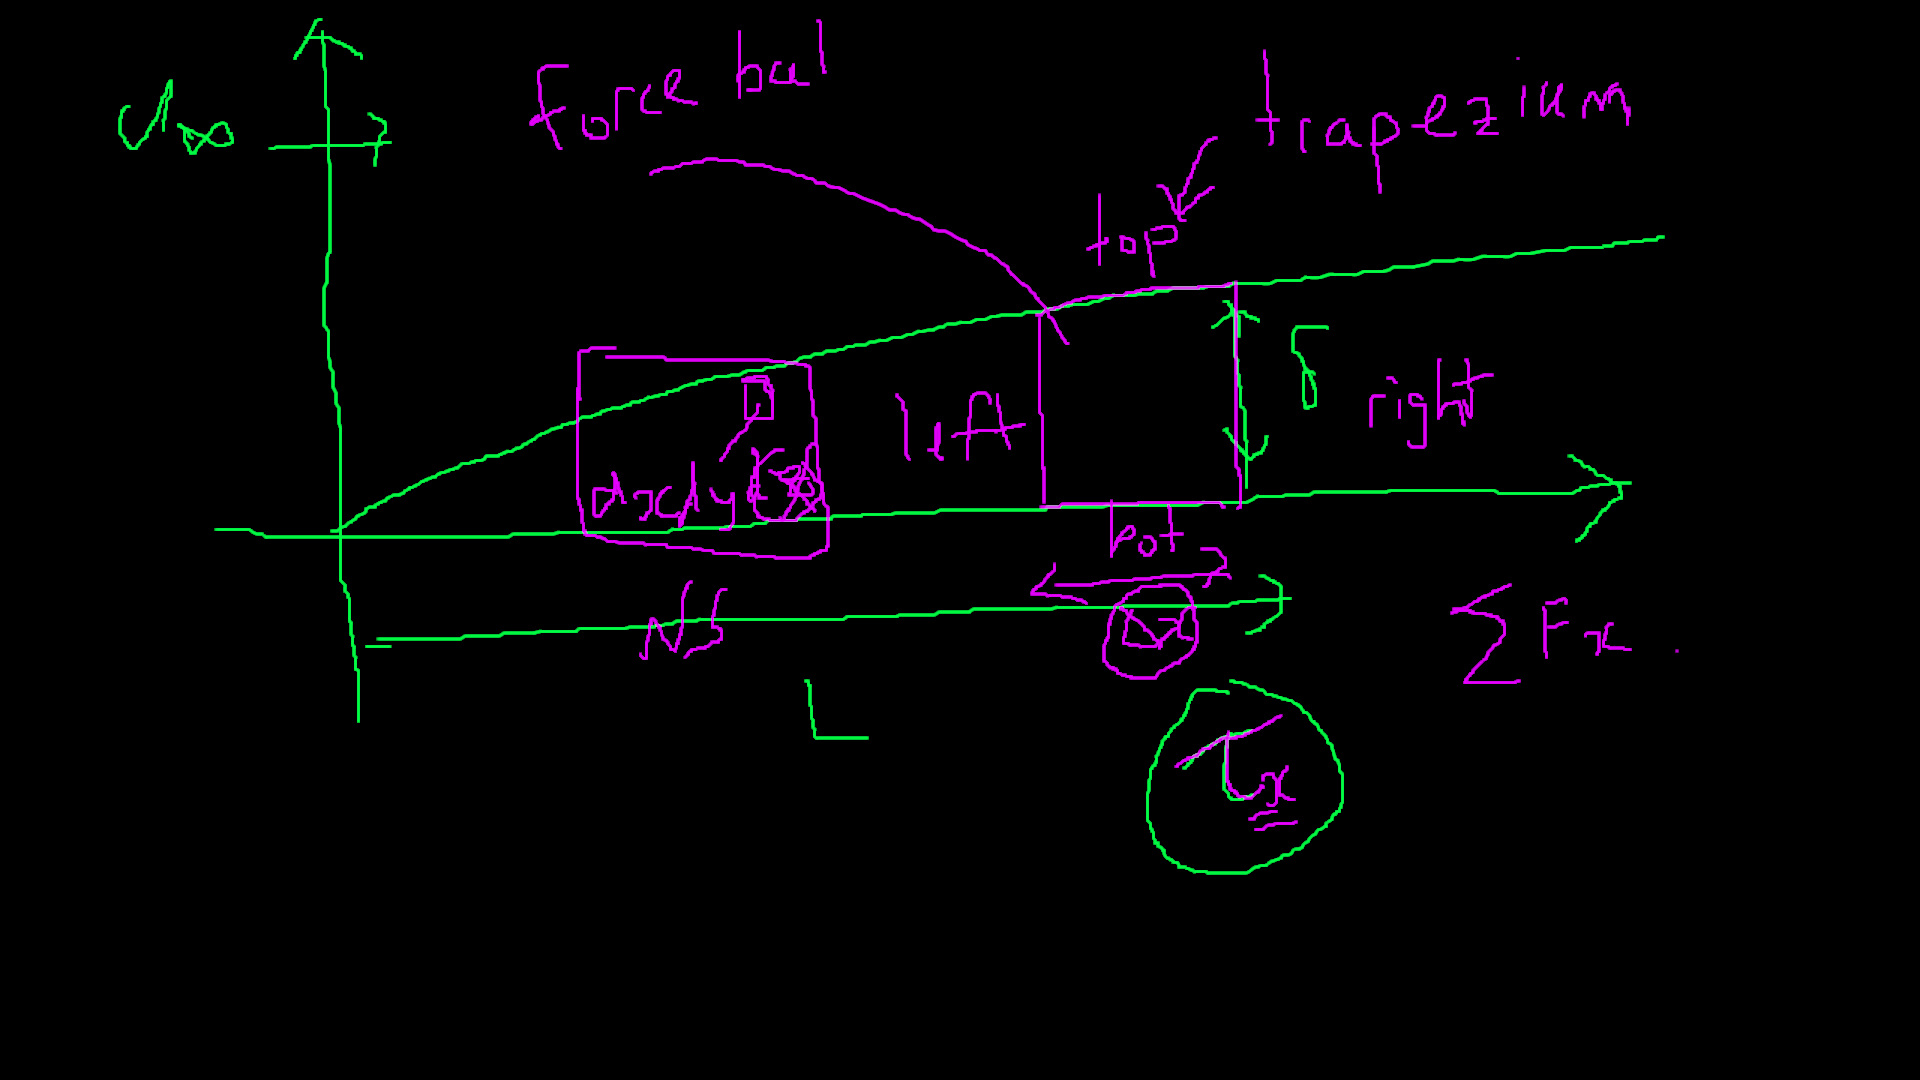
\includegraphics[width=\textwidth]{vonkarman BL.png}
\caption{vonkarman BL}
\label{H and Pb scattering}

\end{figure}

$$\sum F_x = top + bottom + left + right $$


In equilibrium
$$\sum F_x = net \ outflow \ of \ momentum \ in \ CV + accumulation\ term$$

$$accumulation\ term = 0 $$


$$bottom = - \tau_x l_z \Delta x$$

$$left = (P \delta_p l_z)|_x$$

$$right = -(P \delta_p l_z)|_{x+\Delta x}$$

$$top = \frac{P|_x + P|_{x+\Delta x}}{2} (\delta_{x+\Delta x} - \delta_{x}) l_z $$


let's take a look at net outflow of momentum:

left side outflows:

$$-\int \rho u^2 dA |_{x} = - l_z \int_0^{\delta_p} \rho u^2 dy |_x$$

right side outflow:

$$\int \rho u^2 dA |_{x+\Delta x} =  l_z \int_0^{\delta_p} \rho u^2 dy |_{x+\Delta x} $$

Top side outflow:

$$- \dot{m}_{top} u_\infty $$

Now we need an expression for $\dot{m}_{top}$

$$\dot{m}_{top} = \dot{m}_{right} - \dot{m}_{left}$$

$$\dot{m}_{top} = l_z \int_0^{\delta_p |_{x+\Delta x}} \rho u |_{x+ \Delta x}dy -  l_z \int_0^{\delta_p |_{x}} \rho u |_{x}dy$$

total momentum outlflow

$$net \ outflow \ of  \ momentum = - l_z \int_0^{\delta_p} \rho u^2 dy |_x +  l_z \int_0^{\delta_p} \rho u^2 dy |_{x+\Delta x} - \dot{m}_{top} u_\infty  $$

$$net \ outflow \ of  \ momentum = - l_z \int_0^{\delta_p} \rho u^2 dy |_x +  l_z \int_0^{\delta_p} \rho u^2 dy |_{x+\Delta x} $$

$$ - ( l_z \int_0^{\delta_p |_{x+\Delta x}} \rho u |_{x+ \Delta x}dy -  l_z \int_0^{\delta_p |_{x}} \rho u |_{x}dy) u_\infty  $$

Sum of forces:

$$\sum F_x = -\tau_x l_z \Delta x + (P \delta_p l_z)|_x - (P \delta_p l_z)|_{x+\Delta x} + \frac{P|_x + P|_{x+\Delta x}}{2} (\delta_{x+\Delta x} - \delta_{x}) $$

Equating both:

$$-\tau_x l_z \Delta x + (P \delta_p l_z)|_x -  (P \delta_p l_z)|_{x+\Delta x} + \frac{P|_x + P|_{x+\Delta x}}{2} (\delta_{x+\Delta x} - \delta_{x}) l_z= $$

$$= - l_z \int_0^{\delta_p} \rho u^2 dy |_x +  l_z \int_0^{\delta_p} \rho u^2 dy |_{x+\Delta x} $$

$$ - ( l_z \int_0^{\delta_p |_{x+\Delta x}} \rho u |_{x+ \Delta x}dy -  l_z \int_0^{\delta_p |_{x}} \rho u |_{x}dy) u_\infty  $$

Cancel out $l_z$

$$-\tau_x \Delta x + (P \delta_p )|_x -  (P \delta_p )|_{x+\Delta x} + \frac{P|_x + P|_{x+\Delta x}}{2} (\delta_{x+\Delta x} - \delta_{x}) = $$

$$= - \int_0^{\delta_p} \rho u^2 dy |_x +   \int_0^{\delta_p} \rho u^2 dy |_{x+\Delta x} $$

$$ - (  \int_0^{\delta_p |_{x+\Delta x}} \rho u |_{x+ \Delta x}dy -  \int_0^{\delta_p |_{x}} \rho u |_{x}dy) u_\infty  $$

Divide by $\Delta x$ limit $\Delta x \rightarrow 0 $


$$-\tau_x   + \frac{(P \delta_p )|_x -  (P \delta_p )|_{x+\Delta x}}{\Delta x}  + \frac{1}{2} \frac{P|_x + P|_{x+\Delta x}}{\Delta x} (\delta_p|_{x+\Delta x} - \delta_p|_{x}) = $$

$$=  \frac{- \int_0^{\delta_p} \rho u^2 dy |_x +   \int_0^{\delta_p} \rho u^2 dy |_{x+\Delta x}}{\Delta x}  $$

$$ - \frac{1}{\Delta x} (  \int_0^{\delta_p |_{x+\Delta x}} \rho u |_{x+ \Delta x}dy -  \int_0^{\delta_p |_{x}} \rho u |_{x}dy) u_\infty  $$

Take limits first:

$$ \lim_{\Delta x \rightarrow 0} [-\tau_x   + \frac{(P \delta_p )|_x -  (P \delta_p )|_{x+\Delta x}}{\Delta x}  + \frac{1}{2} \frac{P|_x + P|_{x+\Delta x}}{\Delta x} (\delta_p|_{x+\Delta x} - \delta_p|_{x})] = $$

$$=  \lim_{x \rightarrow 0}[ \frac{- \int_0^{\delta_p} \rho u^2 dy |_x +   \int_0^{\delta_p} \rho u^2 dy |_{x+\Delta x}}{\Delta x}  $$

$$ - \frac{1}{\Delta x} (  \int_0^{\delta_p |_{x+\Delta x}} \rho u |_{x+ \Delta x}dy -  \int_0^{\delta_p |_{x}} \rho u |_{x}dy) u_\infty]   $$

$$ \lim_{\Delta x \rightarrow 0} [-\tau_x   + \frac{(P \delta_p )|_x -  (P \delta_p )|_{x+\Delta x}}{\Delta x}  + \frac{1}{2} \frac{P|_x + P|_{x+\Delta x}}{\Delta x} (\delta_p|_{x+\Delta x} - \delta_p|_{x})] = $$

$$=  \frac{\partial }{\partial x} \int_0^{\delta_p} \rho u^2 dy    - \frac{\partial }{\partial x} (u_\infty \int_0^{\delta_p } \rho u dy )   $$

[careless mistake here! last term on the right hand side (RHS)]

$$ \lim_{\Delta x \rightarrow 0} [-\tau_x   + \frac{(P \delta_p )|_x -  (P \delta_p )|_{x+\Delta x}}{\Delta x}  + \frac{1}{2} \frac{P|_x + P|_{x+\Delta x}}{\Delta x} (\delta_p|_{x+\Delta x} - \delta_p|_{x})] = $$

$$=  \frac{\partial }{\partial x} \int_0^{\delta_p} \rho u^2 dy    - u_\infty \frac{\partial }{\partial x} ( \int_0^{\delta_p } \rho u dy )   $$

Left hand side...

$$ -\tau_x   +  \lim_{\Delta x \rightarrow 0} [\frac{(P \delta_p )|_x -  (P \delta_p )|_{x+\Delta x}}{\Delta x}  + \frac{1}{2} \frac{P|_x + P|_{x+\Delta x}}{\Delta x} (\delta_p|_{x+\Delta x} - \delta_p|_{x})] = $$

$$=  \frac{\partial }{\partial x} \int_0^{\delta_p} \rho u^2 dy    - u_\infty  \frac{\partial }{\partial x} (\int_0^{\delta_p } \rho u dy )   $$

look in the terms inside the limit:

$$\lim_{\Delta x \rightarrow 0} [\frac{(P \delta_p )|_x -  (P \delta_p )|_{x+\Delta x}}{\Delta x}  + \frac{1}{2} \frac{P|_x + P|_{x+\Delta x}}{\Delta x} (\delta_p|_{x+\Delta x} - \delta_p|_{x})] $$


$$=\lim_{\Delta x \rightarrow 0} [\frac{(P \delta_p )|_x -  (P \delta_p )|_{x+\Delta x}}{\Delta x}  + \frac{1}{2} \frac{2P|_x + P|_{x+\Delta x} - P|_x}{\Delta x} (\delta_p|_{x+\Delta x} - \delta_p|_{x})] $$

$$=\lim_{\Delta x \rightarrow 0} [\frac{(P \delta_p )|_x -  (P \delta_p )|_{x+\Delta x}}{\Delta x}  + \frac{1}{2} \frac{ P|_{x+\Delta x} - P|_x}{\Delta x} (\delta_p|_{x+\Delta x} - \delta_p|_{x}) + P|_x \frac{1}{\Delta x} (\delta_p|_{x+\Delta x} - \delta_p|_{x})] $$


$$= P \frac{\partial \delta_p}{\partial x} + \lim_{\Delta x \rightarrow 0} [\frac{(P \delta_p )|_x -  (P \delta_p )|_{x+\Delta x}}{\Delta x}  + \frac{1}{2} \frac{ P|_{x+\Delta x} - P|_x}{\Delta x} (\delta_p|_{x+\Delta x} - \delta_p|_{x})] $$

$$= P \frac{\partial \delta_p}{\partial x} + \lim_{\Delta x \rightarrow 0} [\frac{(P \delta_p )|_x -  (P \delta_p )|_{x+\Delta x}}{\Delta x}  + \frac{1}{2} \frac{ P|_{x+\Delta x} - P|_x}{\Delta x} (\delta_p|_{x+\Delta x} ) - \frac{1}{2}\delta_p|_{x} \frac{ P|_{x+\Delta x} - P|_x }{\Delta x}  ] $$

$$= P \frac{\partial \delta_p}{\partial x} + \lim_{\Delta x \rightarrow 0} [\frac{(P \delta_p )|_x -  (P \delta_p )|_{x+\Delta x}}{\Delta x}  + \frac{1}{2} \frac{ \delta_p|_{x+\Delta x} P|_{x+\Delta x} - \delta_p|_{x+\Delta x} P|_x}{\Delta x} - \frac{1}{2} \frac{\delta_p|_{x} P|_{x+\Delta x} -\delta_p|_{x} P|_x }{\Delta x}  ] $$

$$= P \frac{\partial \delta_p}{\partial x} + \lim_{\Delta x \rightarrow 0} [\frac{(P \delta_p )|_x -  (P \delta_p )|_{x+\Delta x}}{\Delta x}  + \frac{1}{2} \frac{ (\delta_p P)_{x+\Delta x} - \delta_p|_{x+\Delta x} P|_x}{\Delta x} - \frac{1}{2} \frac{\delta_p|_{x} P|_{x+\Delta x} -(\delta_p P)|_x }{\Delta x}  ] $$

$$= P \frac{\partial \delta_p}{\partial x} + \lim_{\Delta x \rightarrow 0} [ \frac{( 1.5 P \delta_p )|_x -  0.5 (P \delta_p )|_{x+\Delta x}}{\Delta x}  - \frac{1}{2} \frac{ \delta_p|_{x+\Delta x} P|_x}{\Delta x} - \frac{1}{2} \frac{\delta_p|_{x} P|_{x+\Delta x}}{\Delta x}  ] $$

$$= P \frac{\partial \delta_p}{\partial x} + \lim_{\Delta x \rightarrow 0} [ \frac{(P \delta_p)|_x + (0.5 P \delta_p )|_x -  0.5 (P \delta_p )|_{x+\Delta x}}{\Delta x}  - \frac{1}{2} \frac{ \delta_p|_{x+\Delta x} P|_x}{\Delta x} - \frac{1}{2} \frac{\delta_p|_{x} P|_{x+\Delta x}}{\Delta x}  ] $$

$$= P \frac{\partial \delta_p}{\partial x} -0.5 \frac{\partial P\delta_p}{\partial x} + \lim_{\Delta x \rightarrow 0} [ \frac{(P \delta_p)|_x}{\Delta x}  - \frac{1}{2} \frac{ \delta_p|_{x+\Delta x} P|_x}{\Delta x} - \frac{1}{2} \frac{\delta_p|_{x} P|_{x+\Delta x}}{\Delta x}  ] $$


$$= P \frac{\partial \delta_p}{\partial x} - 0.5 \frac{\partial P\delta_p}{\partial x} + \lim_{\Delta x \rightarrow 0} [ \frac{(P \delta_p)|_x}{\Delta x}  - \frac{1}{2} \frac{ \delta_p|_{x+\Delta x} P|_x - \delta_p |_x P|_x + \delta_p |_x P_x }{\Delta x} - \frac{1}{2} \frac{\delta_p|_{x} P|_{x+\Delta x}}{\Delta x}  ] $$


$$= P \frac{\partial \delta_p}{\partial x} -0.5 \frac{\partial P\delta_p}{\partial x} + \lim_{\Delta x \rightarrow 0} [ \frac{0.5(P \delta_p)|_x}{\Delta x}  - \frac{1}{2} \frac{ \delta_p|_{x+\Delta x} P|_x - \delta_p |_x P|_x}{\Delta x} - \frac{1}{2} \frac{\delta_p|_{x} P|_{x+\Delta x}}{\Delta x}  ] $$

$$= P \frac{\partial \delta_p}{\partial x} -0.5 \frac{\partial P\delta_p}{\partial x} - 0.5 P \frac{\partial \delta_p}{\partial x} + \lim_{\Delta x \rightarrow 0} [  - \frac{1}{2} \frac{\delta_p|_{x} P|_{x+\Delta x} - \delta_p |_x P|_x}{\Delta x}  ] $$

$$= P \frac{\partial \delta_p}{\partial x} -0.5 \frac{\partial P\delta_p}{\partial x} - 0.5 P \frac{\partial \delta_p}{\partial x}  -  0.5 \delta_p \frac{\partial P}{\partial x}$$

$$=P \frac{\partial \delta_p}{\partial x} - 0.5 P \frac{\partial \delta_p}{\partial x}  - 0.5\delta_p \frac{\partial P}{\partial x} - 0.5 P \frac{\partial \delta_p}{\partial x}  -  0.5 \delta_p \frac{\partial P}{\partial x}$$

$$=  - 0.5\delta_p \frac{\partial P}{\partial x} -  0.5 \delta_p \frac{\partial P}{\partial x}$$

$$=  -  \delta_p \frac{\partial P}{\partial x}$$

Substitute back in...
$$ -\tau_x -  \delta_p \frac{\partial P}{\partial x} =  \frac{\partial }{\partial x} \int_0^{\delta_p} \rho u^2 dy    - u_\infty  \frac{\partial }{\partial x} (\int_0^{\delta_p } \rho u dy )   $$

$$ -  \delta_p \frac{\partial P}{\partial x} = \tau_x + \frac{\partial }{\partial x} \int_0^{\delta_p} \rho u^2 dy    - u_\infty \frac{\partial }{\partial x} ( \int_0^{\delta_p } \rho u dy )   $$

Only assumption is that

$$u_\infty = constant \ w.r.t \ y$$

Bernoulli's equation

[careless mistake here...]

I wrote
$$\frac{\partial P}{\partial x} = \rho u_\infty \frac{\partial u_\infty}{\partial x}$$

When it's actually
$$-\frac{\partial P}{\partial x} = \rho u_\infty \frac{\partial u_\infty}{\partial x}$$

we can assume this holds with or without flat plate...

Substitute back in:

$$ \delta_p \rho u_\infty \frac{\partial u_\infty}{\partial x} = \tau_x + \frac{\partial }{\partial x} \int_0^{\delta_p} \rho u^2 dy    -u_\infty \frac{\partial }{\partial x} ( \int_0^{\delta_p } \rho u dy )   $$

constant density fluid:

$$ \delta_p  u_\infty \frac{\partial u_\infty}{\partial x} =  \frac{\tau_x}{\rho} + \frac{\partial }{\partial x} \int_0^{\delta_p}  u^2 dy    -u_\infty \frac{\partial }{\partial x} ( \int_0^{\delta_p } u dy )   $$

We'll need to tidy all this up:

2 tricks to use to tidy up equation

$$\frac{\partial}{\partial x} u_\infty^2 \delta_p =  \delta_p  u_\infty \frac{\partial u_\infty}{\partial x} + u_\infty \frac{\partial \delta_p u_\infty}{\partial x} $$

$$\delta_p = \int_0^{\delta_p} 1 dy  = \int_0^{\delta_p} dy$$

$$\frac{\partial}{\partial x} u_\infty^2  \int_0^{\delta_p} dy =  \int_0^{\delta_p} dy  u_\infty \frac{\partial u_\infty}{\partial x} + u_\infty \frac{\partial \int_0^{\delta_p} dy u_\infty}{\partial x} $$

$$ \delta_p  u_\infty \frac{\partial u_\infty}{\partial x}  = \frac{\partial}{\partial x} u_\infty^2  \delta_p -u_\infty \frac{\partial \delta_p u_\infty}{\partial x} $$

substitute back in:

$$  \frac{\partial}{\partial x} u_\infty^2  \delta_p  -u_\infty \frac{\partial \delta_p  u_\infty}{\partial x}= \frac{\tau_x}{\rho} + \frac{\partial }{\partial x} \int_0^{\delta_p}  u^2 dy    - u_\infty\frac{\partial }{\partial x} ( \int_0^{\delta_p } u dy )   $$




[continue from here... note careless mistake]

1. Partial derivative wrong for mass balance 
2. I think i said you can swap derivatives and integrals freely, do not do that. Leibniz's rule applied rather carelessly (don't carelessly swap integrals, leave it as $\delta_p$ first)
3. Bernoulli's equation sign is wrong

$$ \frac{\partial}{\partial x} u_\infty^2  \delta_p  -u_\infty \frac{\partial \delta_p  u_\infty}{\partial x}= \frac{\tau_x}{\rho} + \frac{\partial }{\partial x} \int_0^{\delta_p}  u^2 dy    - u_\infty\frac{\partial }{\partial x} ( \int_0^{\delta_p } u dy )   $$


Combine terms:

$$  \frac{\partial}{\partial x} [u_\infty^2  \delta_p - \int_0^{\delta_p}  u^2 dy  ]  +u_\infty \frac{\partial }{\partial x} [ \int_0^{\delta_p } u dy -\delta_p  u_\infty ] = \frac{\tau_x}{\rho}  $$

Replace $\delta_p$ with: 
$$\delta_p = \int_0^{\delta_p} 1 dy  = \int_0^{\delta_p} dy$$
Assume 

$$\frac{\partial}{\partial y } U_\infty = 0$$

$$ \frac{\partial}{\partial x} [ \int_0^{\delta_p}u_\infty^2  dy - \int_0^{\delta_p} u^2 dy  ]  +u_\infty \frac{\partial }{\partial x} [-\int_0^{\delta_p } u_\infty dy + \int_0^{\delta_p } u dy ] = \frac{\tau_x}{\rho}  $$


$$ \frac{\partial}{\partial x}   \int_0^{\delta_p} (u_\infty^2 - u^2) dy  + u_\infty \frac{\partial }{\partial x} \int_0^{\delta_p} (u -  u_\infty )dy = \frac{\tau_x}{\rho}  $$


get a $a^2-b^2 = (a+b)(a-b)$ expansion


$$ \frac{\partial}{\partial x}   \int_0^{\delta_p} ( u_\infty - u) (u+u_\infty) dy + u_\infty \frac{\partial }{\partial x} \int_0^{\delta_p} (u -  u_\infty )dy = \frac{\tau_x}{\rho}  $$

separate out first integral

$$  \frac{\partial}{\partial x}   \int_0^{\delta_p} ( u_\infty - u) u dy  + \frac{\partial}{\partial x}   \int_0^{\delta_p} ( u_\infty - u) u_\infty dy + u_\infty \frac{\partial }{\partial x} \int_0^{\delta_p} (u -  u_\infty )dy = \frac{\tau_x}{\rho}  $$

Notice the last integral, it is the odd one out in terms of derivatives, let's change it using product rule

$$ u_\infty \frac{\partial }{\partial x} \int_0^{\delta_p} (u -  u_\infty )dy $$
$$= \frac{\partial }{\partial x}[u_\infty \int_0^{\delta_p} (u -  u_\infty )dy] -( \frac{\partial u_\infty}{\partial x}) \int_0^{\delta_p} (u -  u_\infty )dy$$

We can substitute this back in:

$$  \frac{\partial}{\partial x}   \int_0^{\delta_p} ( u_\infty - u) u dy  + \frac{\partial}{\partial x}   \int_0^{\delta_p} ( u_\infty - u) u_\infty dy  +\frac{\partial }{\partial x}[u_\infty \int_0^{\delta_p} (u -  u_\infty )dy]] $$

$$-( \frac{\partial u_\infty}{\partial x}) \int_0^{\delta_p} (u - u_\infty )dy = \frac{\tau_x}{\rho}  $$

Now we can bring the $u_\infty$ into the dy integral

$$  \frac{\partial}{\partial x}   \int_0^{\delta_p} ( u_\infty - u) u dy  + \frac{\partial}{\partial x}   \int_0^{\delta_p} ( u_\infty - u) u_\infty dy  +\frac{\partial }{\partial x}[\int_0^{\delta_p} u_\infty (u -  u_\infty )dy]] $$

$$-( \frac{\partial u_\infty}{\partial x}) \int_0^{\delta_p} (u - u_\infty )dy = \frac{\tau_x}{\rho}  $$


Terms inside cancel each other out...

$$  \frac{\partial}{\partial x}   \int_0^{\delta_p} ( u_\infty - u) u dy  + \frac{\partial}{\partial x}   \int_0^{\delta_p} ( u_\infty - u) u_\infty dy  -\frac{\partial }{\partial x}[\int_0^{\delta_p} u_\infty ( u_\infty - u)dy]] $$

$$-( \frac{\partial u_\infty}{\partial x}) \int_0^{\delta_p} (u - u_\infty )dy = \frac{\tau_x}{\rho}  $$

bring minus sign in,


$$  \frac{\partial}{\partial x}   \int_0^{\delta_p} ( u_\infty - u) u dy +( \frac{\partial u_\infty}{\partial x}) \int_0^{\delta_p} ( u_\infty - u )dy = \frac{\tau_x}{\rho}  $$

Final form of Von Karman equation:

$$ \frac{\tau_x}{\rho} = ( \frac{\partial u_\infty}{\partial x}) \int_0^{\delta_p} ( u_\infty - u ) \ dy  + \frac{\partial}{\partial x}   \int_0^{\delta_p} u( u_\infty - u) \ dy $$

\section{Solutions to BL for Von Karman}

Pohlhausen solution:

$$u = a + b y + c y^2 + d y^3$$

Consider boundary conditions

no slip:

$$u = 0 \ at \  y=0$$
This implies a=0

$$u = b y + c y^2 + d y^3$$

$$y \rightarrow \infty \  u = u_\infty$$

$$y \rightarrow \delta_p \  u \rightarrow u_\infty$$

approximation:
$$y = \delta_p \  u =  u_\infty$$

\begin{equation}
u_\infty = b \delta_p + c \delta_p^2 + d \delta_p^3
\end{equation}

exact:
$$y = \delta_p \  u = 0.99 u_\infty$$


inviscid flow near $\delta_p$ and shear stress is 0 there

$$\frac{\partial u}{\partial y} = 0 \ at \ y = \delta_p$$
$$\frac{\partial u}{\partial y} = b + 2c y + 3d y^2$$
\begin{equation}
0 = b + 2c \delta_p + 3d \delta_p^2
\end{equation}

Last BC:

$$\frac{\partial^2 u}{\partial y^2} = 0 \ at \ y = 0$$

in other words

$$\frac{ \partial \tau_x}{\partial y}= 0$$

$$\frac{\partial^2 u}{\partial y^2} = 2c + 6d y$$

$$0 = 2c $$

$$c=0$$

2 equations left:

$$0 = b + 3d \delta_p^2$$
$$u_\infty = b \delta_p + d \delta_p^3$$

$$b = -3d \delta_p^2$$


$$u_\infty = -3 d\delta_p^3 + d \delta_p^3$$

$$u_\infty = -2d\delta_p^3 $$

\begin{equation}
d= - \frac{u_\infty}{2\delta_p^3}
\end{equation}

$$b= -3 \delta_p^2 (- \frac{u_\infty}{2\delta_p^3}) $$

\begin{equation}
b = \frac{3}{2 \delta_p} u_\infty
\end{equation}

Pohlhausen velocity profile

$$u = \frac{3}{2 \delta_p} u_\infty y  - \frac{u_\infty}{2\delta_p^3} y^3  $$

if we wanted to include the 0.99 $u_\infty$

$$u = 0.99 (\frac{3}{2 \delta_p} u_\infty y  - \frac{u_\infty}{2\delta_p^3} y^3 ) $$

substitute back in von karman equation

$$ \frac{\tau_x}{\rho} = ( \frac{\partial u_\infty}{\partial x}) \int_0^{\delta_p} ( u_\infty - u ) \ dy  + \frac{\partial}{\partial x}   \int_0^{\delta_p} u( u_\infty - u) \ dy $$

under constant freestream velocity:

$$ \frac{\tau_x}{\rho} =  \frac{\partial}{\partial x}   \int_0^{\delta_p} u( u_\infty - u) \ dy $$

$$ \frac{\tau_x}{\rho} =  \frac{\partial}{\partial x}   \int_0^{\delta_p} (\frac{3}{2 \delta_p} u_\infty y  - \frac{u_\infty}{2\delta_p^3} y^3)( u_\infty - (\frac{3}{2 \delta_p} u_\infty y  - \frac{u_\infty}{2\delta_p^3} y^3)) \ dy $$

note that $\delta_p$ only changes with x, not y

$$ \frac{\tau_x}{\rho} =  \frac{\partial}{\partial x}   (\frac{3}{2 \delta_p} u_\infty \frac{\delta_p^2}{2}  - \frac{u_\infty}{2\delta_p^3} \frac{\delta_p^4}{4})( u_\infty \delta_p - (\frac{3}{2 \delta_p} u_\infty \frac{\delta_p^2}{2} - \frac{u_\infty}{2\delta_p^3} \frac{\delta_p^4}{4}))  $$

$$ \frac{\tau_x}{\rho} =  \frac{\partial}{\partial x}   (\frac{3}{2 \delta_p} u_\infty \frac{\delta_p^2}{2}  - \frac{u_\infty}{2\delta_p^3} \frac{\delta_p^4}{4})( u_\infty \delta_p - \frac{3}{2 \delta_p} u_\infty \frac{\delta_p^2}{2} + \frac{u_\infty}{2\delta_p^3} \frac{\delta_p^4}{4})  $$


$$ \frac{\tau_x}{\rho} =  \frac{\partial}{\partial x}   ( u_\infty \delta_p (\frac{3}{2 \delta_p} u_\infty \frac{\delta_p^2}{2}  - \frac{u_\infty}{2\delta_p^3} \frac{\delta_p^4}{4}) - \frac{3}{2 \delta_p} u_\infty \frac{\delta_p^2}{2} (\frac{3}{2 \delta_p} u_\infty \frac{\delta_p^2}{2}  - \frac{u_\infty}{2\delta_p^3} \frac{\delta_p^4}{4})+ \frac{u_\infty}{2\delta_p^3} \frac{\delta_p^4}{4}(\frac{3}{2 \delta_p} u_\infty \frac{\delta_p^2}{2}  - \frac{u_\infty}{2\delta_p^3} \frac{\delta_p^4}{4}))  $$


$$ \frac{\tau_x}{\rho} =  \frac{\partial}{\partial x}   ( (\frac{3}{2 \delta_p} u_\infty^2 \frac{\delta_p^3}{2} - \frac{u_\infty^2}{2\delta_p^3} \frac{\delta_p^5}{4}) $$


$$ - \frac{3}{2 \delta_p} u_\infty \frac{\delta_p^2}{2} (\frac{3}{2 \delta_p} u_\infty \frac{\delta_p^2}{2}  - \frac{u_\infty}{2\delta_p^3} \frac{\delta_p^4}{4})+ \frac{u_\infty}{2\delta_p^3} \frac{\delta_p^4}{4}(\frac{3}{2 \delta_p} u_\infty \frac{\delta_p^2}{2}  - \frac{u_\infty}{2\delta_p^3} \frac{\delta_p^4}{4}))  $$

(not very efficient...)

The more efficient method:

$$ \frac{\tau_x}{\rho} =  \frac{\partial}{\partial x}   \int_0^{\delta_p} (\frac{3}{2} u_\infty \frac{y}{\delta_p}  - \frac{u_\infty}{2} (\frac{y}{\delta_p} )^3)( u_\infty - (\frac{3}{2} u_\infty (\frac{y}{\delta_p} )  - \frac{u_\infty}{2} (\frac{y}{\delta_p} )^3)) \ dy $$

$$ \frac{\tau_x}{\rho} =  u_\infty^2 \frac{\partial}{\partial x}   \int_0^{\delta_p} (\frac{3}{2} \frac{y}{\delta_p}  - \frac{1}{2} (\frac{y}{\delta_p} )^3)( 1 - (\frac{3}{2} (\frac{y}{\delta_p} )  - \frac{1}{2} (\frac{y}{\delta_p} )^3)) \ dy $$


Use chain rule:

$$\frac{dy}{dx} = \frac{dy}{du} \frac{du}{dx}$$

$$dy = \frac{dy}{du} du$$

$$u = \frac{y}{\delta_p}$$

$$du = \frac{1}{\delta_p} dy$$

$$\delta_p du = dy$$

Change integration variable:

$$u = \frac{y}{\delta_p}$$
$$ \frac{\tau_x}{\rho} =  u_\infty^2 \frac{\partial}{\partial x}  \delta_p \int_0^1 (\frac{3}{2} \frac{y}{\delta_p}  - \frac{1}{2} (\frac{y}{\delta_p} )^3)( 1 - (\frac{3}{2} (\frac{y}{\delta_p} )  - \frac{1}{2} (\frac{y}{\delta_p} )^3)) \ d\frac{y}{\delta_p} $$

$$ \frac{\tau_x}{\rho} =  u_\infty^2 \frac{\partial}{\partial x}  \delta_p \int_0^1 (\frac{3}{2} u  - \frac{1}{2} (u)^3)( 1 - (\frac{3}{2} u )  + \frac{1}{2} (u)^3) \ du $$

$$ \frac{\tau_x}{\rho}|_{wall} = 0.139286 u_\infty^2 \frac{\partial}{\partial x}  \delta_p  $$

From textbook:

$$ \frac{\tau_x}{\rho}|_{wall} = \frac{39}{280} u_\infty^2 \frac{\partial}{\partial x}  \delta_p  $$

Substitute in shear stress

$$\tau_x|_{wall} = \rho \nu \frac{\partial u}{\partial y}|_{y=0}$$

shear stress

$$\frac{\partial u}{\partial y} = \frac{3}{2 \delta_p} u_\infty + 3 (-\frac{u_\infty}{2 \delta_p^3}) y^2$$

at y=0 we find $\tau_x|_{y=0}$

$$\frac{\partial u}{\partial y} = \frac{3}{2 \delta_p} u_\infty $$

$$\frac{\tau_x |_{wall}}{\rho} = \nu \frac{\partial u}{\partial y}|_{y=0} = \nu \frac{3}{2 \delta_p} u_\infty $$

Substitute back:
$$ \nu \frac{3}{2 \delta_p} u_\infty  = \frac{39}{280} u_\infty^2 \frac{\partial}{\partial x}  \delta_p  $$

$$ \nu \frac{1}{ \delta_p}   = \frac{13}{140} u_\infty \frac{\partial}{\partial x}  \delta_p  $$

$$ \nu \frac{1}{ \delta_p}   = \frac{13}{140} u_\infty \frac{d}{d x}  \delta_p  $$

$$ \nu \frac{140}{13}  dx = u_\infty  \delta_p  d \delta_p  $$

$$ \nu \frac{140}{13} \int_0^x dx = u_\infty \int_0^{\delta_p (x)} \delta_p  d \delta_p  $$

In proper math notation, we have to use dummy variables

$$ \nu \frac{140}{13} \int_0^x dx' = u_\infty \int_0^{\delta_p (x)} \delta_p'  d \delta_p'  $$

Integrating:

$$ \nu \frac{140}{13} x= u_\infty \frac{\delta_p (x)^2}{2}  $$
$$ \nu \frac{280}{13} x= u_\infty \delta_p (x)^2  $$

$$\delta_p (x) = \sqrt{\frac{280}{13} \frac{\nu x}{u_\infty}}$$

$$\delta_p (x) = \sqrt{\frac{280}{13} \frac{\nu}{u_\infty x} x^2}$$

$$\delta_p (x) \frac{1}{x} = \sqrt{\frac{280}{13} \frac{\nu}{u_\infty x} }$$


$$ \frac{\delta_p (x)}{x} = \sqrt{\frac{280}{13} \frac{1}{Re_x} }$$


$$ \frac{\delta_p (x)}{x} =  4.64095 \sqrt{ \frac{1}{Re_x} }$$

Where $Re_x = \frac{u_\infty x}{\nu}$

To get shear stress

$$\frac{\tau_x|_{wall}}{\rho} = \nu \frac{3}{2 \delta_p} u_\infty $$

$$\frac{\tau_x|_{wall}}{\rho} = \nu \frac{3}{2* 4.64095 \sqrt{ \frac{1}{Re_x} } x} u_\infty $$

Skin coefficient of friction (local)

$$C_{fx} \equiv \frac{\tau_x |_{wall}}{\frac{1}{2} \rho u_\infty^2}$$

$$C_{fx} \equiv \frac{2}{ u_\infty^2} \nu \frac{3}{2* 4.64095 \sqrt{ \frac{1}{Re_x} } x} u_\infty$$


$$C_{fx} \equiv \frac{0.6464}{ u_\infty} \nu \frac{1}{\sqrt{ \frac{1}{Re_x} } x} $$
$$C_{fx} \equiv \frac{0.6464}{ 1}  \frac{1}{\sqrt{ \frac{1}{Re_x} } Re_x} $$

$$C_{fx} \equiv \frac{0.6464}{ \sqrt{Re_x}}  $$

Average skin friction coefficient:

$$C_{fL} \equiv \frac{1}{L} \int_0^L C_{fx} dx$$

$$C_{fL} \equiv \frac{1}{L} \int_0^L\frac{0.6464}{ \sqrt{Re_x}} dx$$

$$C_{fL} \equiv \frac{1}{L} \int_0^L\frac{0.6464 \sqrt{\nu}}{\sqrt{u_\infty x} } dx$$

$$C_{fL} \equiv \frac{0.6464 \sqrt{\nu}}{\sqrt{ u_\infty }L} \int_0^L\frac{1 }{ \sqrt{x} } dx$$

$$C_{fL} \equiv \frac{0.6464 \sqrt{\nu}}{\sqrt{ u_\infty }L} \int_0^L\frac{1 }{ \sqrt{x} } dx$$

$$C_{fL} \equiv \frac{0.6464 \sqrt{\nu}}{\sqrt{ u_\infty }L} 2 \sqrt{L}$$

$$C_{fL} \equiv \frac{0.6464 \sqrt{\nu}}{\sqrt{ u_\infty }L} 2 \sqrt{L}$$

$$C_{fL} \equiv \frac{1.2928 \sqrt{\nu}}{\sqrt{ u_\infty L}}  $$

$$C_{fL} \equiv \frac{1.2928 }{\sqrt{Re_L}}  $$


\subsubsection{Solution Comparison to Similarity Solution}

\paragraph{Von Karman Results (approximate solution)}
$$ \frac{\delta_p (x)}{x} =   \frac{4.64095 }{\sqrt{Re_x} }$$


$$C_{fx} \equiv \frac{0.6464}{ \sqrt{Re_x}}  $$

$$C_{fL} \equiv \frac{1.2928 }{\sqrt{Re_L}}  $$

\paragraph{Blasius Results (Exact solution) }


$$ \frac{\delta_p (x)}{x} =   \frac{5}{\sqrt{Re_x} }$$


$$C_{fx} \equiv \frac{0.664}{ \sqrt{Re_x}}  $$

$$C_{fL} \equiv \frac{1.328}{\sqrt{Re_L}}  $$

7.2\% off for BL thickness, and 3\% off for skin friction coeff.
Pretty good!

This shows that Von Karman method is pretty good, if you can't use Blasius results 

\begin{verbatim}
Welty, J., Rorrer, G. L., & Foster, D. G. (2014). 
Fundamentals of momentum, heat, and mass transfer. John Wiley & Sons.
\end{verbatim}

\section{Resources Online}


\begin{verbatim}
http://web.mit.edu/fluids-modules/www/highspeed_flows/ver2/bl_Chap2.pdf
https://community.dur.ac.uk/suzanne.fielding/teaching/BLT/sec3.pdf

for Von Karman
https://nptel.ac.in/content/storage2/courses/112104118/lecture-29/29-3_momentum.htm
\end{verbatim}

\part{Github Repo}
\begin{verbatim}
https://github.com/theodoreOnzGit/heatTransferTheory_YouTube
\end{verbatim}

Look under convection heat transfer...

\end{document}

%% template for graphics
%
%\begin{figure}[H]
%\centering
%
%\includegraphics[width=\textwidth]{Q10_compare.png}
%\caption{H (blue) and Pb scattering inelastic (red) and elastic (green)}
%\label{H and Pb scattering}
%
%\end{figure}